\documentclass[a4paper]{article}
\usepackage[utf8]{inputenc}


%=-=-=-=-=-=-=-=-=-=-=-=-=-=-=-=-=-=-=-=-=-=-=-=-=-=-=-=-=-=-=-=-=-=-=-=-=-=-=-=-
% PREAMBLE
%=-=-=-=-=-=-=-=-=-=-=-=-=-=-=-=-=-=-=-=-=-=-=-=-=-=-=-=-=-=-=-=-=-=-=-=-=-=-=-=-

%%%%%%%%%%%%%%%%%%%%%%%%%%%%%%%%%%%%%%%%%%%%%%%%%%%%%%%%%%%%%%%%%%%%%
% Important styling notes
%%
% For now, to include img.jpg in img/path/to/img.jpg, just use:
% path/to/img.jpg - for details see style.tex
%=-=-=-=-=-=-=-=-=-=-=-=-=-=-=-=-=-=-=-=-=-=-=-=-=-=-=-=-=-=-=-=-=-=-=-=-=-=-=-=-
% Packages
%%
%\usepackage{fullpage} % Package to use full page
\usepackage[top=1in,bottom=1in,left=1in,right=0.7in,heightrounded]{geometry}

\usepackage{parskip}                    % Package to tweak paragraph skipping
\usepackage{amsmath}                    % standard
\usepackage{amssymb}                    % standard - Double R symbol etc.
\usepackage{hyperref}
\usepackage{amsthm}                     % standard - theorem, definition, etc.
\usepackage{multicol}                   % multiple columns for numbering
\usepackage{enumitem}                   % standard - enumerate styles
\usepackage[utf8]{inputenc}
\usepackage{scrextend}                  % indentation
\usepackage{graphicx}                   % standard - add figures
\usepackage{float}                      % standard - figure position, use [H] option
\usepackage{pifont}                     % symbols
\usepackage{gensymb}                    % degree symbol \degree
\usepackage{xcolor}                     % bg color
\hypersetup{
    colorlinks,
    linkcolor={black!50!black},
    citecolor={blue!50!black},
    urlcolor={blue!80!black}
}
\usepackage{framed}                     % bg color
\usepackage[T1]{fontenc}                % small caps
\usepackage{sectsty}                    % headings colour
\usepackage{mathtools}                  % Loads amsmath
\usepackage{amsthm,thmtools,xcolor}     % coloured theorem
\usepackage[toc,page]{appendix}         % reference to appendix
%\usepackage{titlesec}                   % change chapter, section, etc. formats
\usepackage{xifthen}                    % if, else
\usepackage{etoolbox}
% format numbering in theorem, lemma, etc. environment
\AtBeginEnvironment{theorem}{\setlist[enumerate, 1]{font=\upshape,  wide=0.5em, before=\leavevmode}}
\AtBeginEnvironment{lemma}{\setlist[enumerate, 1]{font=\upshape,  wide=0.5em, before=\leavevmode}}
\usepackage[letterspace=150]{microtype} % \textls{<letterspaced text>} % 0 <= letterspace <= 1000, 1000 = M space
\usepackage{letltxmacro}                % renew commands?
\usepackage{minted}                     % package to list code
    % otherwise minted goes off the page
    \setmintedinline{breaklines}
\usepackage{subfig}
\usepackage{eso-pic}                    % title page bg pic
\usepackage{varwidth}
\PassOptionsToPackage{svgnames}{xcolor}
\usepackage{fontawesome}                % \faQuestionCircle
\usepackage{marvosym}                   %\Pointinghand
\usepackage{mdframed}                   % easy outline frames
\usepackage[many]{tcolorbox}            % colour box for theorem styles
\usepackage{array,booktabs,calc} % table figs and text
\usepackage{comment}                    % \begin{comment}
\usepackage{fancyhdr}                   % page headings
\usepackage{mdframed}                   % boxes
\usepackage[backend=biber,sorting=none,style=ieee]{biblatex}
\usepackage{caption}
%%% caption options {
%\DeclareCaptionFont{white}{\color{white}}
\DeclareCaptionFormat{listing}{\colorbox{magenta!30!gray}{\parbox{\textwidth}{#1#2#3}}}
\captionsetup[lstlisting]{format=listing,labelfont={bf,small},textfont=small,skip=-1pt}
%%% }
\addbibresource{bibliography.bib}
\usepackage{url}
\usepackage{textcomp}
\usepackage[makeroom]{cancel}            % crossed symbols
\usepackage{algorithm}
\usepackage[noend]{algpseudocode}
\usepackage{tikz}
\usetikzlibrary{arrows.meta,positioning,quotes} % arrows and nodes in tikz
\usepackage{marginnote}
\usepackage{pgfplots}
\usepackage{pstricks-add,pst-slpe}  % for fancy tikz arrows
%\usepackage{titlesec}                   % title style
\usepackage{lmodern}                    % a font
\usepackage{titletoc} % Required for manipulating the table of contents
\usepackage{titlesec} % Allows customization of titles
\usepackage{fouriernc} % Use the New Century Schoolbook font
\usepackage{booktabs} % things in page margins
\usepackage{stmaryrd } % \varoast
\usepackage{listings} % code listings
\usepackage{longtable} % table across multiple pages
\usepackage{styles/nasm/lang}  % include custom language for NASM assembly.
\usepackage{styles/nasm/style} % include custom style for NASM assembly.



%% extra comments that I don't know where they belong:
% list of ding tags: http://willbenton.com/wb-images/pifont.pdf

%=-=-=-=-=-=-=-=-=-=-=-=-=-=-=-=-=-=-=-=-=-=-=-=-=-=-=-=-=-=-=-=-=-=-=-=-=-=-=-=-
% Colours for various things
%%


\definecolor{shadecolor}{rgb}{1.,0.933,0.96} % bg color, r,g,b <= 1
\definecolor{medium_blue}{RGB}{60,125,190}
\definecolor{dark_blue}{RGB}{25,60,85}
\definecolor{dark_red}{RGB}{77,16,16}
\definecolor{LightPink}{rgb}{0.92.,0.8,0.84} % bg color, r,g,b <= 1
\definecolor{LighterPink}{rgb}{1.,0.94,0.97} % bg color, r,g,b <= 1
\definecolor{LightestPink}{rgb}{1.,0.95,0.99} % bg color, r,g,b <= 1
\definecolor{DarkestPink}{rgb}{0.36, 0.0, 0.18}
\definecolor{DarkerPink}{rgb}{0.41, 0.0, 0.21}
\definecolor{DarkPink}{rgb}{0.55, 0.05, 0.37}
\definecolor{lightestestpink}{RGB}{255,248,252}
\definecolor{codegray}{rgb}{0.5,0.5,0.5}
\definecolor{codegrayblue}{rgb}{0.35,0.35,0.47}



%=-=-=-=-=-=-=-=-=-=-=-=-=-=-=-=-=-=-=-=-=-=-=-=-=-=-=-=-=-=-=-=-=-=-=-=-=-=-=-=-
% Define my own theorem styles
%%

% "base" styles
\declaretheoremstyle[
  headfont=\color{DarkPink}\bfseries,
  bodyfont=\itshape,
]{colored}

\declaretheoremstyle[
  headfont=\color{DarkPink}\bfseries,
  bodyfont=\normalfont,
]{colored_upright}

% theorems (corollaries, etc) themselves, inherit from my style above
% Usage:
% \begin{theorem} \end{theorem}, \begin{lemma} \end{lemma}, ...
\declaretheorem[
	numberwithin=section,
 	style=colored,
	name=\textsc{Theorem},
]{theorem}

\tcolorboxenvironment{theorem}{
  boxrule=0pt,
  boxsep=2pt,
  colback={magenta!25!white},
  colframe=DarkPink,
  enhanced jigsaw, 
  borderline west={2pt}{0pt}{DarkPink},
  sharp corners,
  before skip=5pt,
  after skip=5pt,
  breakable,
  right=0mm % for equations
}

\declaretheorem[
	numberwithin=section,
 	style=colored,
	name=\textsc{Corollary},
]{corollary}

\tcolorboxenvironment{corollary}{
  boxrule=0pt,
  boxsep=1pt,
  colback={magenta!10!white},
  colframe=DarkPink,
  enhanced jigsaw, 
  borderline west={2pt}{0pt}{DarkPink},
  sharp corners,
  before skip=5pt,
  after skip=5pt,
  breakable,
  right=0mm % for equations
}

\declaretheorem[
	numberwithin=section,
	style=colored,
	name=\textsc{Lemma},
]{lemma}

\tcolorboxenvironment{lemma}{
  boxrule=0pt,
  boxsep=1pt,
  colback={magenta!10!white},
  colframe=DarkPink,
  enhanced jigsaw, 
  borderline west={2pt}{0pt}{DarkPink},
  sharp corners,
  before skip=5pt,
  after skip=5pt,
  breakable,
  right=0mm % for equations
}

\declaretheorem[
	numberwithin=section,
	style=colored,
	name=\textsc{Definition},
]{definition}

\tcolorboxenvironment{definition}{
  boxrule=0pt,
  boxsep=1pt,
  colback={magenta!25!white},
  colframe=DarkPink,
  enhanced jigsaw, 
  borderline west={2pt}{0pt}{DarkPink},
  sharp corners,
  before skip=5pt,
  after skip=5pt,
  breakable,
  right=0mm % for equations
}

\declaretheorem[
	numberwithin=section,
  	style=colored,
  	name=\textsc{Example},
]{exmp}

\declaretheorem[
	numberwithin=section,
  	style=colored,
  	name=\textsc{Solution},
]{soln}

%%% code listings
\lstdefinestyle{code1}{
    backgroundcolor=\color{lightestestpink},   
    commentstyle=\color{codegrayblue},
    keywordstyle=\color{DarkerPink},
    numberstyle=\tiny\color{codegray},
    stringstyle=\color{black!40!cyan},
    basicstyle=\small\ttfamily,
    breakatwhitespace=false,
    breaklines=true,        
    captionpos=t,             
    keepspaces=true,        
    numbers=left,           
    numbersep=5pt,
    showspaces=false, 
    showstringspaces=false,
    showtabs=false,
    tabsize=4
}

\lstset{style=code1}

%=-=-=-=-=-=-=-=-=-=-=-=-=-=-=-=-=-=-=-=-=-=-=-=-=-=-=-=-=-=-=-=-=-=-=-=-=-=-=-=-
% Headers (size, font, colour)
%%




\makeatletter
\renewcommand{\@seccntformat}[1]{\llap{\textcolor{DarkestPink}{\csname the#1\endcsname}\hspace{1em}}}                    
\renewcommand{\section}{\@startsection{section}{1}{\z@}
{-4ex \@plus -1ex \@minus -.4ex}
{1ex \@plus.2ex }
{\normalfont\large\sffamily\bfseries\textcolor{DarkestPink}}}
\renewcommand{\subsection}{\@startsection {subsection}{2}{\z@}
{-3ex \@plus -0.1ex \@minus -.4ex}
{0.5ex \@plus.2ex }
{\normalfont\sffamily\bfseries\textcolor{DarkestPink}}}
\renewcommand{\subsubsection}{\@startsection {subsubsection}{3}{\z@}
{-2ex \@plus -0.1ex \@minus -.2ex}
{.2ex \@plus.2ex }
{\normalfont\small\sffamily\bfseries\textcolor{DarkestPink}}}                        


%=-=-=-=-=-=-=-=-=-=-=-=-=-=-=-=-=-=-=-=-=-=-=-=-=-=-=-=-=-=-=-=-=-=-=-=-=-=-=-=-
% Numberings, counters and spacings
%%
\numberwithin{equation}{section} % section number in eq/s
\setlength{\jot}{7pt} % spacing in split, gathered env/s



%% Custom examples
%% Output - Example 1,2,...
\newcounter{example}
\newenvironment{example}[1][]{\refstepcounter{example}\par\medskip
   \textbf{Example~\theexample. #1} \rmfamily}{\medskip}
%%%%%%%%%%%% End of unused %%%%%%%%%%%%



%=-=-=-=-=-=-=-=-=-=-=-=-=-=-=-=-=-=-=-=-=-=-=-=-=-=-=-=-=-=-=-=-=-=-=-=-=-=-=-=-
% Paths
%%
\graphicspath{ {./img/} } % figures' path - can look up files directly from there


%=-=-=-=-=-=-=-=-=-=-=-=-=-=-=-=-=-=-=-=-=-=-=-=-=-=-=-=-=-=-=-=-=-=-=-=-=-=-=-=-
% User defined macros (math mode)
%%


% Curly braces under text. Usage: \myunderbrace{upper}{lower}
\newcommand{\myunderbrace}[2]{\mathrlap{\underbrace{\phantom{#1}}_{#2}} #1}
\newcommand{\setR}{\mathbb{R}} % \ouble R
\newcommand{\setRn}{\mathbb{R}^n} %  double R^n
\newcommand{\setN}{\mathbb{N}} % double N
\newcommand{\setZ}{\mathbb{Z}} % double Z
\let\oldemptyset\emptyset
\let\emptyset\varnothing % nice - looking empty set symbol
\newcommand{\fancyN}{\mathcal{N}} % null space
\newcommand{\fancyR}{\mathcal{R}} % range

\newcommand{\bx}{\textbf{x}}
\newcommand{\by}{\textbf{y}}
\newcommand{\bb}{\textbf{b}}
\newcommand{\bA}{\textbf{A}}
\newcommand{\bB}{\textbf{B}}
\newcommand{\bI}{\textbf{I}}
% double bars as in norm
\newcommand{\norm}[1] {\lVert #1 \rVert} 
\newcommand{\trans}[1]{#1^{\top}}

\newcommand{\mean}[1]{\bar{#1}}
\newcommand{\var}{\sigma^2}

\newcommand{\partdevx}[1]{\frac{\partial #1}{\partial x}}
\newcommand{\partdevxx}[1]{\frac{\partial #1}{\partial x}}
\newcommand{\partdevxn}[1]{\frac{\partial^n #1}{\partial x^n}}
\newcommand{\partdevy}[1]{\frac{\partial #1}{\partial x}}
\newcommand{\partdevyy}[1]{\frac{\partial #1}{\partial y}}
\newcommand{\partdevyn}[1]{\frac{\partial^n #1}{\partial y^n}}

% text above = symbol
\newcommand{\overeq}[1]{\ensuremath{\stackrel{#1}=}} 
\newcommand{\greatersmaller}{%
  \mathrel{\ooalign{\raisebox{.6ex}{$>$}\cr\raisebox{-.6ex}{$<$}}}
} % greater and smaller symbols on top of each other, same line

%=-=-=-=-=-=-=-=-=-=-=-=-=-=-=-=-=-=-=-=-=-=-=-=-=-=-=-=-=-=-=-=-=-=-=-=-=-=-=-=-
% User defined macros (non math)

\newcommand{\qedblack}{$\hfill\blacksquare$} % black square end of line
\newcommand{\qedwhite}{\hfill \ensuremath{\Box}} % white square end of line
\newcommand{\hquad}{\hskip0.5em\relax}% half quad space
%\newcommand{\TODO}{\textcolor{red}{\bf TODO!}\;}

\newcommand{\TODO}[1][]{%
    \ifthenelse{\equal{#1}{}}{\textcolor{red}{\bf TODO!}\;}{\textcolor{red}{\textbf {TODO:} #1}\; }%
}
\newcommand{\B}[1]{\textbf{\textup{#1}}} % bold and upright
\renewcommand{\labelitemi}{\scriptsize$\textcolor{DarkPink}{\blacksquare}$} % itemize - squares instead of bullets
\newcommand{\emphasis}[1]{\textls{#1}}

\LetLtxMacro{\originaleqref}{\eqref}
\renewcommand{\eqref}{Eq.~\originaleqref}
\renewcommand*{\eqref}[1]{Eq.~\originaleqref{#1}}





% background images
%%%%%%%
\newcommand\BackgroundPic{%
\put(0,0){%
\parbox[b][\paperheight]{\paperwidth}{%
\vfill
%\centering

\includegraphics[width=0.125\paperwidth,height=\paperheight,%
]{img/background_02.png}% use ,keepaspectratio
\vfill
}}}
%%%%%%%
% end of background image
%%%%%%%%%%%%%% my own frame
\newmdenv[topline=false,bottomline=false]{leftrightbox}
%%%%%%%%%%%%% end
%%%%%%%%%%%%% my own comment
\newcommand{\mycomment}[1]{\begin{leftrightbox}\Pointinghand~\textbf{Comment:}~#1 \end{leftrightbox}}
%%%%%%%%%%%%% end
% my custom note https://tex.stackexchange.com/questions/301993/create-custom-note-environment-with-tcolorbox
\newmdenv[
    topline=false,
    bottomline=false,
    rightline=false,
    innerrightmargin=0pt
]{siderule}
\newenvironment{mynote}%
    {\begin{siderule}\textbf{\Pointinghand~Note:}}
    {\end{siderule}}
%%%%%%%%%%%%% my own box
\newcommand{\boxone}[1]{\begin{tcolorbox}[colback = LighterPink,colframe=LightPink]
#1
\end{tcolorbox}}
%%%%%%%%%%%%% end

\let\oldemptyset\emptyset
\let\emptyset\varnothing
%algorithmic
\algdef{SE}[DOWHILE]{Do}{doWhile}{\algorithmicdo}[1]{\algorithmicwhile\ #1}%






\begin{document}
%=-=-=-=-=-=-=-=-=-=-=-=-=-=-=-=-=-=-=-=-=-=-=-=-=-=-=-=-=-=-=-=-=-=-=-=-=-=-=-=-
% GLOBAL STYLES (DOCUMENT SCOPE)
%=-=-=-=-=-=-=-=-=-=-=-=-=-=-=-=-=-=-=-=-=-=-=-=-=-=-=-=-=-=-=-=-=-=-=-=-=-=-=-=-
% caption: Figure 1 -> <bold> Fig. 1 </bold>
\captionsetup[figure]{labelfont={bf},labelformat={default},labelsep=period,name={Fig.}}


%=-=-=-=-=-=-=-=-=-=-=-=-=-=-=-=-=-=-=-=-=-=-=-=-=-=-=-=-=-=-=-=-=-=-=-=-=-=-=-=-
% TITLE PAGE
%=-=-=-=-=-=-=-=-=-=-=-=-=-=-=-=-=-=-=-=-=-=-=-=-=-=-=-=-=-=-=-=-=-=-=-=-=-=-=-=-
%%%%%%%%%%%%%%%%%%%%%%%%%%%%%%%%%%%%%%%%%
% Formal Book Title Page
% LaTeX Template
% Version 2.0 (23/7/17)
%
% This template was downloaded from:
% http://www.LaTeXTemplates.com
%
% Original author:
% Peter Wilson (herries.press@earthlink.net) with modifications by:
% Vel (vel@latextemplates.com)
%
% License:
% CC BY-NC-SA 3.0 (http://creativecommons.org/licenses/by-nc-sa/3.0/)
% 
% This template can be used in one of two ways:
%
% 1) Content can be added at the end of this file just before the \end{document}
% to use this title page as the starting point for your document.
%
% 2) Alternatively, if you already have a document which you wish to add this
% title page to, copy everything between the \begin{document} and
% \end{document} and paste it where you would like the title page in your
% document. You will then need to insert the packages and document 
% configurations into your document carefully making sure you are not loading
% the same package twice and that there are no clashes.
%
%%%%%%%%%%%%%%%%%%%%%%%%%%%%%%%%%%%%%%%%%

%----------------------------------------------------------------------------------------
%	PACKAGES AND OTHER DOCUMENT CONFIGURATIONS
%----------------------------------------------------------------------------------------



%----------------------------------------------------------------------------------------
%	TITLE PAGE
%----------------------------------------------------------------------------------------



\begin{titlepage} % Suppresses headers and footers on the title page

	\centering % Centre everything on the title page
	
	\scshape % Use small caps for all text on the title page
	
	\vspace*{\baselineskip} % White space at the top of the page
	
	%------------------------------------------------
	%	Title
	%------------------------------------------------
	
	\rule{\textwidth}{1.6pt}\vspace*{-\baselineskip}\vspace*{2pt} % Thick horizontal rule
	\rule{\textwidth}{0.4pt} % Thin horizontal rule
	
	\vspace{0.75\baselineskip} % Whitespace above the title
	
	{\LARGE COMPUTER VISION NOTES\\ \Large OBJECT LOCALISATION AND TRACKING\\} % Title
	
	\vspace{0.75\baselineskip} % Whitespace below the title
	
	\rule{\textwidth}{0.4pt}\vspace*{-\baselineskip}\vspace{3.2pt} % Thin horizontal rule
	\rule{\textwidth}{1.6pt} % Thick horizontal rule
	
	\vspace{2\baselineskip} % Whitespace after the title block
	
	%------------------------------------------------
	%	Subtitle
	%------------------------------------------------
	My personal notes on
	
	\vspace*{3\baselineskip} % Whitespace under the subtitle
	
	Object Localisation Techniques; Colour Matching, Mean Shift Tracking, Optical Flow, Lukas Kanade 
	
	\vspace*{3\baselineskip} % Whitespace under the subtitle
	
	%------------------------------------------------
	%	Editor(s)
	%------------------------------------------------
	
	By
	
	\vspace{0.5\baselineskip} % Whitespace before the editors
	
	{\normalfont \Large \mintinline{latex}{0xLeo} (\url{github.com/0xleo}) \\} % Editor list
	
	\vspace{0.5\baselineskip} % Whitespace below the editor list
	
	%\textit{The University of California \\ Berkeley} % Editor affiliation
	
	\vfill % Whitespace between editor names and publisher logo
	
	%------------------------------------------------
	%	Publisher
	%------------------------------------------------
	
	
	\vspace{0.3\baselineskip} % Whitespace under the publisher logo
	
	\today % Date
	
	{DRAFT X.YY} % Draft version
	{\\Missing: \ldots}

\end{titlepage}

%----------------------------------------------------------------------------------------

%\maketitle



%=-=-=-=-=-=-=-=-=-=-=-=-=-=-=-=-=-=-=-=-=-=-=-=-=-=-=-=-=-=-=-=-=-=-=-=-=-=-=-=-
% MAIN DOCUMENT
%=-=-=-=-=-=-=-=-=-=-=-=-=-=-=-=-=-=-=-=-=-=-=-=-=-=-=-=-=-=-=-=-=-=-=-=-=-=-=-=-
\newpage
\tableofcontents
\newpage



%------------------------------ New section ------------------------------%
\section{Introduction - the $n$-dimensional Gaussian integral}
The problem to solve in this tutorial is to compute the $n$-dimensional Gaussian integral defined as. The $n$-dimensional Gaussian integral has applications in quantum field theory \todo{ref \url{https://link.springer.com/chapter/10.1007/978-1-4612-0209-7_12}} and it's very beautiful to calculate as it combines a lot of linear algebra and multivariable calculus.

Before introducing the integral, it is necessary to remember the definition of a \emphasis{positive definite} matrix.
\begin{definition}[positive definite matrix]
	Let $\bA$ be a $n\times n$ symmetric real matrix. $\bA$ is positive definite iff $\bx\t\bA\bx>0 \;\; \forall \; \bx\in\setR^n - {\bO}$. Equivalently, $\bA$ is positive definite iff all its eigenvalues $\lambda_1,\ldots,\lambda_n$ are strictly positive.
\end{definition}
Proof that these statements are equivalent is obtained by diagonalising matrix $\bA$.

\begin{definition}[$n$-dim. Gaussian integral]
Given a real symmetric and positive-definite matrix $\bA$ of $n\times n$, it is defined as
% ref http://www.weylmann.com/gaussian.pdf
\begin{equation}
	\int_{-\infty}^\infty \int_{-\infty}^\infty \ldots \int_{-\infty}^\infty \exp(-\bx\t \bA \bx) \,dx_1\,dx_2\,\ldots\, dx_n
\end{equation}
\end{definition}

Before attempting to compute it, two techniques are required.
\begin{enumerate}
	\item How to compute 1D Gaussian integrals.
	\item How to perform change of variables in a multivariate integral.
\end{enumerate}



\subsection{Requirements}

\subsubsection{1D Gaussian integral}
\begin{corollary}[Gaussian integral]
\label{cor:gauss_int_1d}
\begin{equation}
	\int_{-\infty}^\infty \exp(-\alpha x^2) = \sqrt{\frac{\pi}{\alpha}}
	\label{eq:gaussian_int_1d}
\end{equation}	
\end{corollary}
\begin{proof}

We start by proving a simpler result for $\alpha=1$; that
	\[
	I := \int_{-\infty}^\infty \exp(-x^2)\, dx = \sqrt{\pi}
	\]
	Changing (renaming) the dummy variable $x$ to $y$:
	\[
	I = \int_{-\infty}^\infty \exp(-y^2)\,dy
	\]
	\[
		\therefore I^2 =\int_{-\infty}^\infty \exp(-y^2)\,dy\int_{-\infty}^\infty \exp(-x^2)\,dx = \int_{-\infty}^\infty\int_{-\infty}^\infty \exp(-x^2-y^2) \,dxdy
	\]
	If we change from Cartesian to polar coordinates in $I^2$, i.e. $x:=\cos(\theta), \; y:=\sin(\theta)$, then $x^2+y^2=r^2$ and $dxdy = rdrd\theta$ \footnote{Proof for $dxdy=rdrd\theta$ in \ref{app:int_change_vars_2d}}. The Cartesian integral limits cover the entire $xy$ plane and so much the polar limits for $r,\theta$. Therefore $r$ ranges from $0$ to $\infty$ and $\theta$ from $0$ to $2\pi$.
	\[
		\therefore I^2 = \int_0^{2\pi}\int_0^{\infty}\exp(-r^2)\,rdrd\theta
	\]
Letting $u:=-r^2\Rightarrow rdr = -u/2$, the limits change $r=0 \Rightarrow u\rightarrow \infty$,\; $r\rightarrow \infty \Rightarrow u \rightarrow -\infty$ and the integral becomes
	\[
		I^2 = - \frac{1}{2} \int_0^{2\pi}\int_0^{-\infty}\exp(u)\,dud\theta = - \frac{1}{2} \int_0^{2\pi}-d\theta = \pi
	\]
To conclude,
	\[
	I = \int_{-\infty}^\infty \exp(-x^2)\, dx = \sqrt{\pi}
	\]
	Finally, substituting in $I$ $x := \sqrt{\alpha} y$, $\alpha>0$, then $dx = \sqrt{\alpha}dy$, therefore
	\begin{gather*}
		\int_{-\infty}^\infty \exp(-\alpha y^2) \sqrt{\alpha}dy = \sqrt{\pi} \Rightarrow \\
		\int_{-\infty}^\infty \exp(-\alpha y^2) dy = \sqrt{\frac{\pi}{\alpha}} 
	\end{gather*}
\end{proof}



\subsubsection{Change of variables in a multivariable integral}

Before introducing the change of variables the change of variables, it is necessary to introduce a scalar quantity called \emphasis{Jacobian}
\begin{definition}[Jacobian]
	% ref: based on https://web.ma.utexas.edu/users/m408m/Display15-10-4.shtml
	For a transformation $\Phi \enskip \setR^m \rightarrow \setR^n : (x_1,\ldots,x_m) \rightarrow \big(f_1(x_1,\ldots,x_n),\ldots,f_n(x_m)\big)$, the \emphasis{Jacobian} is defined as the determinant
	\[
		J = \det\left(
			\begin{bmatrix}
				\frac{\partial f_1}{\partial x_1} & \frac{\partial f_1}{\partial x_2} & \ldots & \frac{\partial f_1}{\partial x_m} \\
				\frac{\partial f_2}{\partial x_2} & \frac{\partial f_2}{\partial x_2} &\ldots & \frac{\partial f_2}{\partial x_m} \\
				\ldots & \ldots & \ddots & \vdots \\
				\frac{\partial f_n}{\partial x_2} & \frac{\partial f_n}{\partial x_2} & \ldots & \frac{\partial f_n}{\partial x_m} \\
			\end{bmatrix}
		\right)	
	\]
	The matrix of partial derivatives in the determinant is called \emphasis{Jacobian matrix}. The latter matrix is often denoted as $\frac{\partial(f_1,\ldots,f_n)}{\partial(x_1,\ldots,x_m)}$ or $\boldsymbol{\nabla} f$ for shorthand.


\end{definition}
\begin{exmp}	
% ref https://web.ma.utexas.edu/users/m408m/Display15-10-4.shtml
	Compute the Jacobian of the transformation from Cartesian to polar coordinates $\Phi: (x,y)\rightarrow (r,\theta)$ defined as $x=r\cos(\theta),\enskip y=r\sin(\theta)$.
\end{exmp}
\begin{soln}
	\[
		J = \det\left(
			\begin{bmatrix}
				\frac{\partial x}{ \partial r} 	 & \frac{\partial x}{\partial \theta} \\ 
				\frac{\partial y}{ \partial r} 	 & \frac{\partial y}{\partial \theta} \\ 
			\end{bmatrix}
		\right)
	\]
Compute partial derivatives
	\begin{gather*}
		\frac{\partial x}{\partial r} = \cos\theta, \qquad \frac{\partial x}{\partial \theta} = -r\sin\theta\\
		\frac{\partial y}{\partial r} = \sin\theta, \qquad \frac{\partial y}{\partial \theta} = r\cos\theta
	\end{gather*}
	Substitute
	\[
		\therefore J = 	\det\left(
			\begin{bmatrix}
				\cos\theta & -r\sin\theta\\
				\sin\theta & r\cos\theta
			\end{bmatrix} 
		\right) = r
	\]
\end{soln}

\begin{lemma}[Change of variables]
	% ref https://web.ma.utexas.edu/users/m408m/Display15-10-4.shtml
	\label{lem:jacobian}
	If an ``1-1'' mapping $\Phi: (x,y)\rightarrow \big(u(x,y), v(x,y)\big)$ sends a region $D$ in $xy$-space to a region $D^*$ in $uv$-space, then
	\begin{equation}
		\int\int_Df(x,y)dxdy = \int\int_{D^*}f(u(x,y), v(x,y))\left| \frac{\partial(u,v)}{\partial(x,y)}  \right| dudv
	\end{equation}
\end{lemma}
Notes:
\begin{enumerate}
	\item Obviously this definition can be generalised in $n$-dimensional mappings but is stated in 2D for clarity.
	\item $\left| . \right|$ denotes absolute value -- we need the absolute Jacobian!
	\item The proof of Lemma \ref{lem:jacobian} in $n$ dimensions is omitted but a neat proof is found in \todo{ref: \url{https://math.stackexchange.com/questions/267267/intuitive-proof-of-multivariable-changing-of-variables-formula-jacobian-withou}}.
\end{enumerate}


\section{Computing the integral}
To reiterate, the integral to compute is the following

\begin{equation*}
	\int_{-\infty}^\infty \int_{-\infty}^\infty \ldots \int_{-\infty}^\infty \exp(-\bx\t \bA \bx) \,dx_1\,dx_2\,\ldots\, dx_n
\end{equation*}
For succinctness, we denote as $D$ the integration space, which is a subspace of $\setR^n$, and the integral as
\[
	\int_D \exp(-\bx\t \bA \bx) \,dx_1\,dx_2\,\ldots\, dx_n
\]
Because $\bA$ is symmetric and real, it's diagonalisable, which means that there exists an orthonormal (therefore symmetric as well) matrix $\textbf{S}$ such that
\[
	\textbf{S}^{-1}\bA \textbf{S}	=\textbf{D} , \quad 
	\textbf{D} = \begin{bmatrix}
	\lambda_1 & &	\\
		& \ddots & \\
	 & & \lambda_n
	\end{bmatrix},\quad
	\lambda_1 > \ldots > \lambda_n > 0
	\tag{1}
\]
Positive eigenvalues $\lambda_i$ are guaranteed as $\bA$ is positive definite. Because $\textbf{S}$ is orthonormal, $\textbf{S}^{-1}= \textbf{S}\t$, therefore Eq. (1) can be rewritten as
\[
	\textbf{S}\t\bA \textbf{S}	=\textbf{D} \Rightarrow \bA = \textbf{S} \textbf{D} \textbf{S}\t
	\tag{2}
\]
The integral is hence rewritten
\[
	I = \int_D \exp(-\bx\t \textbf{S}\textbf{DS}\t \bx) \,dx_1\,dx_2\,\ldots\, dx_n
	\tag{3}
\]
Substitute $\by=\textbf{S}\t\bx$, therefore $\by\t = \bx\t\textbf{S}$. The differentials $dx_1,\ldots,dx_n$ will be transformed to $\left| J \right| dy_1,\ldots, dy_n$ as stated in Lemma \ref{lem:jacobian}, where $J$ is the Jacobian of the linear transform $f(\bx) = \textbf{S}\t \bx$. As proven in \ref{app:jacob_of_lin_transform}, $J = \det(S\t)$. As proven in turn in \ref{app:det_of_ortho_mat}, the determinant of an orthogonal matrix such as $\textbf{S}\t$ is 1. Therefore the new differentials are simply
\[
	dy_1\ldots dy_n = dx_1\ldots dx_n 	
	\tag{4}
\]
Integral $I$ is therefore transformed to
\[
	I = \int_D \exp(-\textbf{y}\t\textbf{D}\textbf{y}) \ dy_1\ldots dy_n
	\tag{5}
\]
The scalar quantity $\by\t \textbf{D} \by$ is called \emphasis{quadratic form} of $\textbf{D}$ and because the latter is diagonal as defined in Eq. (1), it's easy to see that it equals
\[
	\by\t \textbf{D} \by = \lambda_1y_1^2 + \ldots +  \lambda_n y_n^2
	\tag{6}
\]
Substituting Eq. (6) in Eq. (5), the integral is simplified to
\[
	I = \int_D \exp(-\lambda_1y_1^2 - \ldots -\lambda_ny_n^2) dy_1\ldots dy_n
	\tag{7}	
\]
Expanding the integral the $1$-dimensional real subspaces of $\setR^n$ (since D is in $\setR^n$) and breaking the exponential, it can be rewritten as
\[
	I = \int_{D_1} \exp(-\lambda_1 y_1^2)dy_1 \ldots  \int_{D_n} \exp(-\lambda_n y_n^2)dy_n
	\tag{8}
\]
Now each one can be calculated individually. Each sub-integral is a Gaussian one with $\alpha = \lambda_i$, therefore from \eqref{eq:gaussian_int_1d}
\[
	\int_{D_i} \exp(-\lambda_i y_i^2)dy_i = \sqrt{\frac{\pi}{\lambda_i}}, \quad i=1,\ldots,n
	\tag{9}
\]
Finally, from Eq. (8) given Eq. (9)
\[
	\int_{D_1} \exp(-\lambda_1 y_1^2)dy_1 \ldots  \int_{D_n} \exp(-\lambda_n y_n^2)dy_n = \sqrt{ \frac{\pi^n}{\lambda_1\ldots \lambda_n} }
	\tag{10}
\]
Note that the product $\lambda_1\ldots \lambda_n$ is simply the determinant of the diagonal matrix $\textbf{D}$ from Eq. (1), which contains the eigenvalues of $\bA$. Therefore $\lambda_1\ldots \lambda_n = \det(\textbf{D})$. Thus the final result is obtained.
\begin{corollary}[$n-dimensional Gaussian integral$]
	\begin{equation}
	\int_{-\infty}^\infty \int_{-\infty}^\infty \ldots \int_{-\infty}^\infty \exp(-\bx\t \bA \bx) \,dx_1\,dx_2\,\ldots\, dx_n = 
		\sqrt{ \frac{\pi^n}{\det(\textbf{D})} }
	\end{equation}
\end{corollary}


%\subsection{The Gaussian integral with an added linear term}
%
%The integral 
%\[
%	\int_{-\infty}^\infty \int_{-\infty}^\infty \ldots \int_{-\infty}^\infty \exp({-\bx\t\bA\bx + \textbf{J}\t\bx})\ dx_1dx_2\ldots dx_n
%\]
%also often appears in quantum field theory. It is the same as the multivariate Gaussian integral except that the added term $\textbf{Jx}$ appears in the exponential. Once again, $\bA$ is real symmetric of size $n\times n$ and $\bx, \textbf{J} \in \setR^n$.
%
%\textbf{Solution:}
%
%% REF: https://physicspages.com/pdf/Zee%20QFT/Zee%20Notes%20I.02.02%20Gaussian%20integrals%201.pdf
%The way to solve it is very similar with the ``plain'' integral.We diagonalise $\bA$, i.e. 
%\[
%	\bA = \textbf{SDS}\t , \quad \textbf{D} =
%	\begin{bmatrix}
%	\lambda_1 & & \\	
%		& \ddots & \\
%	& & \lambda_n\\
%	\end{bmatrix}, \quad \lambda_1 > \ldots > \lambda_n > 0
%\]
%, where $\textbf{S}$ is orthogonal (a rotation matrix).Therefore the exponent becomes
%\[
%	-\bx\t\bA\bx + \textbf{J}\t \bx	= -\bx\t \textbf{SDS}\t \bx +\textbf{J} \t \bx
%\]
%Similarly to the plain integral, let $\by := \textbf{S}\t \bx \Rightarrow \bx = \textbf{Sy}$, $dy_1\ldots dy_n = dx_1\ldots dx_n$
%\[
%	\therefore	-\bx\t \textbf{SDS}\t \bx +\textbf{Jx}  = -\by\t \textbf{S} \by  + \underbrace{\textbf{J}\t \textbf{S}}_{\textbf{J}'}\by
%\]
%$\textbf{J}$ is a $\setR^n$ vector and $\textbf{S}$ a $n\times n$ matrix, therefore the new vector $\textbf{J}' := \textbf{J}\t\textbf{S} \in \setR^n$. As deduced from the plain integral's solution, 
%\[
%	\by\t \textbf{S} \by = \sum_{i=1}^n \lambda_iy_i^2
%\]
%Furthermore,
%\[
%	\textbf{J}'\by	= \sum_{i=1}^n j'_i y_i
%\]
%Expanding the dot products in the integral
%\begin{gather*}
%	 \int_{-\infty}^\infty \int_{-\infty}^\infty \ldots \int_{-\infty}^\infty \exp({-\bx\t\bA\bx + \textbf{J}\t\bx})\ dx_1dx_2\ldots dx_n = \\
%	 \int_{-\infty}^\infty \int_{-\infty}^\infty \ldots \int_{-\infty}^\infty \exp\Big(\sum_{i=1}^n \lambda_iy_i^2 + \sum_{i=1}^n j'_i y_i
%\Big)\ dy_1dy_2\ldots dy_n =\\
%	 \prod_{i=0}^n \int_{-\infty}^\infty \exp\Big( \sum_{i=1}^n \lambda_i zy_i^2 + \sum_{i=1}^n j'_i y_i\Big)dy_i = \\
%	 \sqrt{ \frac{\pi^n}{\det(\textbf{D})} } \exp\Big(\Big)
%\end{gather*}
%
% http://www.umich.edu/~chem461/Gaussian%20Integrals.pdf
% https://www.youtube.com/watch?v=mcar5MDMd_A
% http://sci.sdsu.edu/johnson/phys410/extra_gauss.pdf
% https://kconrad.math.uconn.edu/blurbs/analysis/gaussianintegral.pdf
% https://en.wikipedia.org/wiki/Common_integrals_in_quantum_field_theory
% https://www.youtube.com/watch?v=g8TWM-FCEgU&t=603s
% http://www-biba.inrialpes.fr/Jaynes/cappe1.pdf
% http://www.weylmann.com/gaussian.pdf
% http://uu.diva-portal.org/smash/get/diva2:731610/FULLTEXT01.pdf

% generalisations in 1D:
%http://www.hep.upenn.edu/~johnda/Papers/GausInt.pdf
% https://www.youtube.com/watch?v=V6ssUIYzzY4



%=-=-=-=-=-=-=-=-=-=-=-=-=-=-=-=-=-=-=-=-=-=-=-=-=-=-=-=-=-=-=-=-=-=-=-=-=-=-=-=-
% References
%=-=-=-=-=-=-=-=-=-=-=-=-=-=-=-=-=-=-=-=-=-=-=-=-=-=-=-=-=-=-=-=-=-=-=-=-=-=-=-=-
\newpage
\printbibliography



%=-=-=-=-=-=-=-=-=-=-=-=-=-=-=-=-=-=-=-=-=-=-=-=-=-=-=-=-=-=-=-=-=-=-=-=-=-=-=-=-
% Appendices
%=-=-=-=-=-=-=-=-=-=-=-=-=-=-=-=-=-=-=-=-=-=-=-=-=-=-=-=-=-=-=-=-=-=-=-=-=-=-=-=-
\newpage
\appendix

\section{Appendices}


% ------------------------ New appendix ------------------------ %
\newpage
\subsection{Lemma proof; Cartesian to polar differentials and $r\,dr\,d\theta$}
\label{app:int_change_vars_2d}

\begin{lemma}
	If we transform from Cartesian to polar coordinates in the integral $I=\int\int_Q f(x,y)\,dx\,dy$ over some area $Q$ by setting $x=r\,\cos(\theta)$, $y=r\,cos(\theta)$, then:
	\begin{equation}
		\int\int_Q f(x,y)\,dx\,dy = \int\int_A f(r\cos(\theta), r\sin(\theta))\, r \, dr\, d\theta
	\end{equation}
\end{lemma}
	\begin{proof}
		% ref https://silo.tips/download/double-integrals-in-polar-coordinates
		Suppose we evaluate the integral over a polar region defined by $\alpha \leq \theta \leq \beta$, $g(\theta) \leq r \leq f(\theta)$, where the curves $f(\theta), g(\theta)$ are contained between two radii $p, q, \quad p<q$. We infinitesimally partition $\theta$ in $\theta_0,\ldots,\theta_m$ and $r$ in $r_0, \ldots, r_n$ (Fig. \ref{fig:polar_partition}).
	\begin{figure}[H]
		\centering
		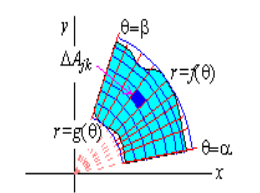
\includegraphics[height=5cm]{img/int_pol_domain.png}
		\caption{Expressing the area as the union of infinitesimal polar partitions.}
		\label{fig:polar_partition}
	\end{figure}
		Then the area $dA$ of each tiny wedge is simply (Fig. \ref{fig:da_wrt_dr})	the difference between the sector from $0$ to $r+dr$ minus the sector from $0$ to $r$:
		\begin{align*}
			dA &= \frac{1}{2}(r+dr)^2d\theta - \frac{1}{2}r^2d\theta  \\
			&= \frac{2r+dr}{2}dr\,d\theta\\
			&= r^*dr\,d\theta 
		\end{align*}
	, where $r^* := \frac{2r+dr}{2}$ is the average radius of the infinitesimal wedge.
	\begin{figure}[H]
		% ref https://math.stackexchange.com/questions/1656814/how-to-prove-dxdy-r-dr-d-theta
		\centering
		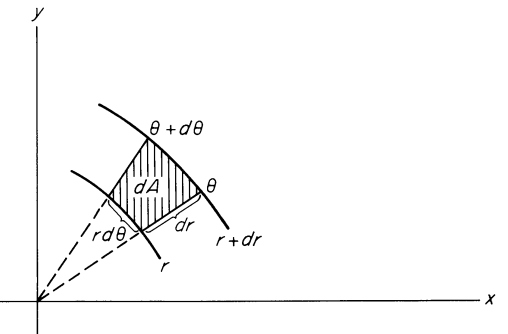
\includegraphics[height=5cm]{img/da_polar_partition.png}
		\caption{Computing $dA$ w.r.t. $dr,\; d\theta$.}
		\label{fig:da_wrt_dr}
	\end{figure}
	\end{proof}
	In general, for the wedge $jk$, its area is:
	\[
		\Delta A_{jk} \approx r_j\Delta r_j \Delta \theta_j
	\]
	If we transform $x$ and $y$ in the polar domain as $x_{jk} = r_j\cos(\theta_k), \; y_{jk} = r_j\sin(\theta_k)$, then the total area expressed by the integral is:
	\begin{gather*}
		\int\int_Q f(x,y)dA =\int\int_Q f(x,y)dxdy  \approx \\
		\sum_{j=1}^{m}\sum_{i=1}^n f(r_i, \theta_j)\Delta A_{ij}
	\end{gather*}
	% ref https://math.stackexchange.com/questions/1656814/how-to-prove-dxdy-r-dr-d-theta
	Taking the limit as $m,n \rightarrow \infty$:
	\[
		\int\int_Q f(x,y)dA = \int_\alpha^\beta\int_{g(\theta)}^{f(\theta)}f(r,\theta)rdrd\theta
	\]

% https://www.youtube.com/watch?time_continue=308&v=2Oo6pdGfLMY&feature=emb_logo
% https://www.youtube.com/watch?time_continue=308&v=2Oo6pdGfLMY&feature=emb_logo

% ------------------------ New appendix ------------------------ %
\newpage
\subsection{Lemma proof; determinant of orthogonal matrix is $\pm 1$}
\label{app:det_of_ortho_mat}

\begin{lemma}
The determinant of an orthogonal matrix is $\pm 1$.
\end{lemma}
\begin{proof}
	
Let $\bU \in \setR^{m\times n}$ be an orthogonal matrix. The columns of an orthogonal matrix are orthonormal, which means
\[
	\bu_i\t\bu_j = 
		\left\{\begin{array}{lr}
			1, & i=j \\
			0, & i \neq j  
			\end{array}
		\right.
\]
for any two columns $\bu_i, \bu_j$. Therefore
\begin{gather*}
	\bU\t\bU = \bI_m	
\end{gather*}
Taking determinant and using their properties:
\begin{gather*}
	\det(\bU)\det(\bU\t) = \det(\bI) \Rightarrow	\\
	\det(\bU)^2 = 1 \Rightarrow \\
	\det(\bU) = \pm 1
\end{gather*}
\end{proof}
% ------------------------ New appendix ------------------------ %
\newpage
\subsection{Proof; Jacobian of linear transform}
\label{app:jacob_of_lin_transform}

% ref http://neutrino.aquaphoenix.com/ReactionDiffusion/SERC5chap7.pdf
\begin{lemma}
Let $\bX\in\setR^n$ and $\bY\in\setR^n$ be two real column vectors. Let also each element of $\bX$ be functionally independent (no element in $\bX$ if a function of element in $\bY$ and vice versa). If $\bY$ is given by the linear transform
	\[
		\bY = \bA\bX,\quad \det(\bA) \neq 0
	\]
, where $\bA = (\alpha_{ij})$ is non-singular $p\times p$ matrix of constants, then
\begin{equation}
	\bY = \bA\bX, \quad \det(\bA) \neq 0 \Rightarrow d\bY = \det(\bA) \, d\bX
\end{equation}
\end{lemma}
\begin{proof}
	We know that when we do change of variables with from $\bX$ to $\bY=f(\bX)$, then the differentials are given by:
	\begin{equation*}
		d\bY = \det(\textbf{J})\, d\bX \tag{1}	
	\end{equation*}
	where $\textbf{J}$ is the Jacobian matrix of $\bY$. For the linear transform $\bY  = \bA\bX$, because $\bX$ and $\bY$ both have length $n$, the Jacobian is given by:
	\begin{equation*}
		\textbf{J} = 	
		\begin{bmatrix}
			\frac{\partial\bY}{\partial x_1} & \frac{\partial\bY}{\partial x_2} & \ldots & \frac{\partial\bY}{\partial x_n} 
		\end{bmatrix} = 
		\begin{bmatrix}
			\frac{\partial\bY_1}{\partial x_1} & \frac{\partial\bY_1}{\partial x_2} & \ldots & \frac{\partial \bY_1}{\partial x_n}	\\
			\frac{\partial\bY_2}{\partial x_1} & \frac{\partial\bY_2}{\partial x_2} & \ldots & \frac{\partial \bY_2}{\partial x_n}	\\
			\vdots & \vdots & \ddots & \vdots \\
			\frac{\partial\bY_n}{\partial x_1} & \frac{\partial\bY_n}{\partial x_2} & \ldots & \frac{\partial \bY_n}{\partial x_n}	
		\end{bmatrix}
		\tag{2}
	\end{equation*}
	However, each element $y_i$ of $\bY$ is given by:
	\[
		y_i = \alpha_{i1}x_1 + \alpha_{i2}x_2 + \ldots + \alpha_{in}x_n, \quad i = 1,\ldots,n
	\]
	Therefore each entry $(i,j)$ of the Jacobian is given by:
	\[
		\frac{\partial y_{i}}{\partial x_j} = \alpha_{ij} \quad \forall \; i = 1,\ldots,n, \quad \forall \; j = 1,\ldots,n
		\tag{3}
	\]
	i.e. $\textbf{J}=\bA$. Therefore Eq. (1) with the aid of Eq. (2), Eq. (3) yields:
	\[
		d\bY = \det(\bA)\,d\bX	
	\]
\end{proof}



% http://neutrino.aquaphoenix.com/ReactionDiffusion/SERC5chap7.pdf
% http://www.mit.edu/~18.338/handouts/handout6.pdf
% mathai jacobian transformations and functions of matrix argumet
% https://math.stackexchange.com/questions/3514146/jacobian-of-an-orthogonal-transformation
% https://www.physicsforums.com/threads/jacobian-of-the-linear-transform-y-ax.401225/
\end{document}
